\documentclass[../main.tex]{subfiles}

\begin{document}

\subsection{Probabilidad continua}
\label{seq:proba:continua}

\paragraph{} Como mencioné antes, estuvimos viendo probabilidades discretas. En esta sección vamos a ver los detalles sobre probabilidades continuas.

Supongamos que queremos realizar un control de calidad en una fábrica de baterías, medimos el tiempo de duración de baterías elegidas al azar y definimos la VA.
\begin{center}
  \(X\): tiempo de duración de una batería
\end{center}

La VA. \(X\) es esencialmente continua (''tiempo''), siendo su rango el intervalo real \([0, \infty)\). Pero supongamos que medimos la duración de la batería en días, es decir ''discretizamos'' el rango de la VA. y su rango se convierte en \(\mathbb{N}_{0}\). Por tratarse de una VA. discreta, su función de probabilidad puntual puede representarse mediante un histograma con área total igual a 1. Si medimos la duración en horas, obtenemos un histograma con mayor número de intervalos de menor longitud cada uno, pero que sigue teniendo área total igual a 1.

Si continuamos aumentando la precisión de la medición (minutos, segundos, décimas de segundos, etc.), obtenemos como límite de los histogramas una curva suave, y la probabilidad de que la duración de la batería se encuentre entre dos valores \(a\) y \(b\) (\(a < b\)) estará dada por el área bajo la curva entre \(a\) y \(b\).

\begin{figure}[H]
  \centering
  \includegraphics[scale=0.3]{continua_histo.png} % TODO: Reemplazar con un gráfico mío
\end{figure}

\paragraph{} Con esta idea, definimos que una VA. \(X\) es \textbf{continua} si existe una función
\begin{gather*}
  f : \mathbb{R} \rightarrow \mathbb{R}^{+} = [0, \infty) \\
  \text{Tal que} \int_{-\infty}^{\infty}f(x)dx = 1
\end{gather*}

Llamada \textbf{función de densidad} de la VA. \(X\) tal que

\begin{gather*}
  P(a \leq X \leq b) = \int_{a}^{b}f(x)dx
\end{gather*}

Es importante resaltar que \(P(X = a) = P(a \leq X \leq a) = 0 \tab \forall a \in \mathbb{R}\).

Se toma la notación \(P(x \leq X) = P(x \leq X \leq \infty)\) y \(P(X \leq x) = P(-\infty \leq X \leq x)\).

\paragraph{} La \textbf{esperanza} de una VA. \(X\) con función de densidad \(f(x)\) está definida como:
\begin{gather*}
  E(X) = \mu_{X} = \int_{-\infty}^{\infty}xf(x)dx \\
  \text{Siempre que} \int_{-\infty}^{\infty}\abs{x}f(x)dx < \infty
\end{gather*}

Una vez definida la esperanza para VA. continuas, se tiene que las otras definiciones y propiedades vistas se valen (varianza, linealidad, etc.).

\paragraph{} Sobre una VA. continua \(X\) con función de densidad \(f(x)\) se definen los \textbf{percentiles}. Donde el percentil (\(100 p\))-ésimo de la distribución de \(X\) es el valor \(x_{p}\) tal que:
\begin{gather*}
  P(X \leq x_{p}) = \int_{-\infty}^{\infty}f(t)dt = p
\end{gather*}

\paragraph{} Es común que las funciones de densidad tengan la estructura:
\begin{gather*}
  f(x) = \begin{cases} g(x) & \text{si } a \leq x \leq b \\ 0 & \text{en otro caso} \end{cases}
\end{gather*}

Para simplificar esa notación se define la función \(I_{A}(x)\) como:
\begin{gather*}
  I_{A}(x) = \begin{cases} 1 & \text{si } x \in A \\ 0 & \text{en otro caso} \end{cases}
\end{gather*}

Y entonces \(f(x) = g(x) \cdot I_{[a, b]}(x)\)

\subsubsection{Distribución Uniforme}

\paragraph{} Se nota \(X \sim U(A, B)\), y describe una VA. que puede tomar cualquier valor en el intervalo \([A, B]\) con igual probabilidad.

Esta es muy usada en programación, ya que con ella se pueden obtener todas las otras distribuciones.

\begin{align*}
  f(x) &= \frac{1}{B-A}I_{[A, B]}(x) \\
  E(X) &= \frac{A+B}{2} \\
  V(X) &= \frac{(B - A)^{2}}{12}
\end{align*}

\subsubsection{Distribución Normal}

\paragraph{} Se nota \(X \sim N(\mu, \sigma^{2})\), y describe una VA. que tiene forma de campana con eje de simetría en \(x = \mu\) y puntos de inflexión en \(x = \mu \pm \sigma\).

\begin{align*}
  f(x) &= \frac{1}{\sqrt{2\pi}\sigma}e^{-\frac{1}{2\sigma^{2}}(x - \mu)^{2}} \\
  E(X) &= \mu \\
  V(X) &= \sigma^{2}
\end{align*}

\begin{figure}[H]
\center
  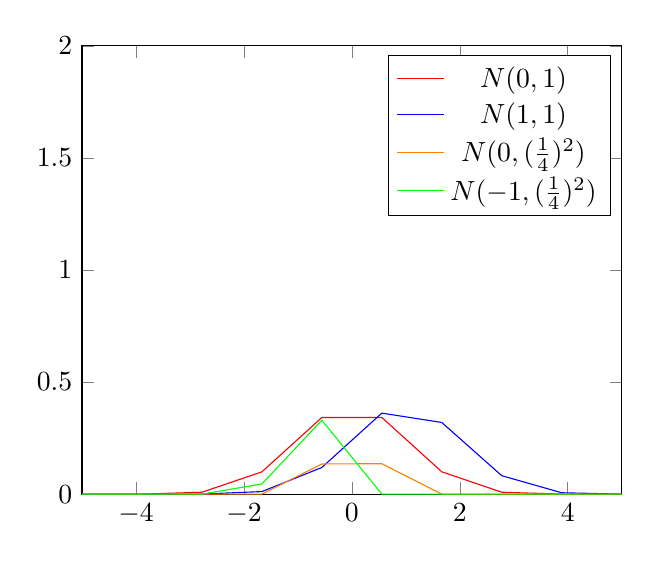
\begin{tikzpicture}
  \begin{axis}[
    xmin=-5, xmax=5,
    ymin=0, ymax=2,
    samples=10, % TODO: More samples
  ]
  
  %\addplot[color=red] { 1 / (sqrt(2 * pi) * SIGMA) * e^(- 1 / (2 * SIGMA^2) * (x - MU)^2) } ;
  \addplot[color=red] { 1 / (sqrt(2 * pi) * 1) * e^(- 1 / (2 * 1^2) * (x - 0)^2) } ;
  \addlegendentry{\(N(0, 1)\)}

  \addplot[color=blue] { 1 / (sqrt(2 * pi) * 1) * e^(- 1 / (2 * 1^2) * (x - 1)^2) } ;
  \addlegendentry{\(N(1, 1)\)}

  \addplot[color=orange] { 1 / (sqrt(2 * pi) * (1/4)) * e^(- 1 / (2 * (1/4)^2) * (x - 0)^2) } ;
  \addlegendentry{\(N(0, (\frac{1}{4})^{2})\)}

  \addplot[color=green] { 1 / (sqrt(2 * pi) * (1/4)) * e^(- 1 / (2 * (1/4)^2) * (x - -1)^2) } ;
  \addlegendentry{\(N(-1, (\frac{1}{4})^{2})\)}

  \end{axis}
  \end{tikzpicture}

  \caption{Diferentes distribuciones normales}
\end{figure}

\paragraph{} Su función de densidad es simétrica respecto de \(\mu\), esto significa que:
\begin{align*}
  f(\mu - x) &= f(\mu + x) & \forall x
\end{align*}

\subsubsection{Distribución Normal Standard}

\paragraph{} Se nota \(Z\) y es la distribución \(N(0, 1)\), su función de distribución se nota \(\phi(z) = P(Z \leq z)\).

Se puede ver que para cualquier \(X \sim N(\mu, \sigma^{2})\) entonces \(\frac{X - \mu}{\sigma} = Z\), por lo que como no se conoce una expresión analítica de la integral de una distribución normal lo que se hace para calcular \(P(X \leq x)\) es tabular los valores de \(\phi\) y tomar \(P(X \leq x) = P(Z \leq \frac{x - \mu}{\sigma})\).
\end{document}
